\documentclass[]{article}
\usepackage{lmodern}
\usepackage{amssymb,amsmath}
\usepackage{ifxetex,ifluatex}
\usepackage{fixltx2e} % provides \textsubscript
\ifnum 0\ifxetex 1\fi\ifluatex 1\fi=0 % if pdftex
  \usepackage[T1]{fontenc}
  \usepackage[utf8]{inputenc}
\else % if luatex or xelatex
  \ifxetex
    \usepackage{mathspec}
  \else
    \usepackage{fontspec}
  \fi
  \defaultfontfeatures{Ligatures=TeX,Scale=MatchLowercase}
\fi
% use upquote if available, for straight quotes in verbatim environments
\IfFileExists{upquote.sty}{\usepackage{upquote}}{}
% use microtype if available
\IfFileExists{microtype.sty}{%
\usepackage{microtype}
\UseMicrotypeSet[protrusion]{basicmath} % disable protrusion for tt fonts
}{}
\usepackage[margin=1in]{geometry}
\usepackage{hyperref}
\hypersetup{unicode=true,
            pdftitle={Regression},
            pdfauthor={Scott Stoltzman},
            pdfborder={0 0 0},
            breaklinks=true}
\urlstyle{same}  % don't use monospace font for urls
\usepackage{color}
\usepackage{fancyvrb}
\newcommand{\VerbBar}{|}
\newcommand{\VERB}{\Verb[commandchars=\\\{\}]}
\DefineVerbatimEnvironment{Highlighting}{Verbatim}{commandchars=\\\{\}}
% Add ',fontsize=\small' for more characters per line
\usepackage{framed}
\definecolor{shadecolor}{RGB}{248,248,248}
\newenvironment{Shaded}{\begin{snugshade}}{\end{snugshade}}
\newcommand{\AlertTok}[1]{\textcolor[rgb]{0.94,0.16,0.16}{#1}}
\newcommand{\AnnotationTok}[1]{\textcolor[rgb]{0.56,0.35,0.01}{\textbf{\textit{#1}}}}
\newcommand{\AttributeTok}[1]{\textcolor[rgb]{0.77,0.63,0.00}{#1}}
\newcommand{\BaseNTok}[1]{\textcolor[rgb]{0.00,0.00,0.81}{#1}}
\newcommand{\BuiltInTok}[1]{#1}
\newcommand{\CharTok}[1]{\textcolor[rgb]{0.31,0.60,0.02}{#1}}
\newcommand{\CommentTok}[1]{\textcolor[rgb]{0.56,0.35,0.01}{\textit{#1}}}
\newcommand{\CommentVarTok}[1]{\textcolor[rgb]{0.56,0.35,0.01}{\textbf{\textit{#1}}}}
\newcommand{\ConstantTok}[1]{\textcolor[rgb]{0.00,0.00,0.00}{#1}}
\newcommand{\ControlFlowTok}[1]{\textcolor[rgb]{0.13,0.29,0.53}{\textbf{#1}}}
\newcommand{\DataTypeTok}[1]{\textcolor[rgb]{0.13,0.29,0.53}{#1}}
\newcommand{\DecValTok}[1]{\textcolor[rgb]{0.00,0.00,0.81}{#1}}
\newcommand{\DocumentationTok}[1]{\textcolor[rgb]{0.56,0.35,0.01}{\textbf{\textit{#1}}}}
\newcommand{\ErrorTok}[1]{\textcolor[rgb]{0.64,0.00,0.00}{\textbf{#1}}}
\newcommand{\ExtensionTok}[1]{#1}
\newcommand{\FloatTok}[1]{\textcolor[rgb]{0.00,0.00,0.81}{#1}}
\newcommand{\FunctionTok}[1]{\textcolor[rgb]{0.00,0.00,0.00}{#1}}
\newcommand{\ImportTok}[1]{#1}
\newcommand{\InformationTok}[1]{\textcolor[rgb]{0.56,0.35,0.01}{\textbf{\textit{#1}}}}
\newcommand{\KeywordTok}[1]{\textcolor[rgb]{0.13,0.29,0.53}{\textbf{#1}}}
\newcommand{\NormalTok}[1]{#1}
\newcommand{\OperatorTok}[1]{\textcolor[rgb]{0.81,0.36,0.00}{\textbf{#1}}}
\newcommand{\OtherTok}[1]{\textcolor[rgb]{0.56,0.35,0.01}{#1}}
\newcommand{\PreprocessorTok}[1]{\textcolor[rgb]{0.56,0.35,0.01}{\textit{#1}}}
\newcommand{\RegionMarkerTok}[1]{#1}
\newcommand{\SpecialCharTok}[1]{\textcolor[rgb]{0.00,0.00,0.00}{#1}}
\newcommand{\SpecialStringTok}[1]{\textcolor[rgb]{0.31,0.60,0.02}{#1}}
\newcommand{\StringTok}[1]{\textcolor[rgb]{0.31,0.60,0.02}{#1}}
\newcommand{\VariableTok}[1]{\textcolor[rgb]{0.00,0.00,0.00}{#1}}
\newcommand{\VerbatimStringTok}[1]{\textcolor[rgb]{0.31,0.60,0.02}{#1}}
\newcommand{\WarningTok}[1]{\textcolor[rgb]{0.56,0.35,0.01}{\textbf{\textit{#1}}}}
\usepackage{graphicx,grffile}
\makeatletter
\def\maxwidth{\ifdim\Gin@nat@width>\linewidth\linewidth\else\Gin@nat@width\fi}
\def\maxheight{\ifdim\Gin@nat@height>\textheight\textheight\else\Gin@nat@height\fi}
\makeatother
% Scale images if necessary, so that they will not overflow the page
% margins by default, and it is still possible to overwrite the defaults
% using explicit options in \includegraphics[width, height, ...]{}
\setkeys{Gin}{width=\maxwidth,height=\maxheight,keepaspectratio}
\IfFileExists{parskip.sty}{%
\usepackage{parskip}
}{% else
\setlength{\parindent}{0pt}
\setlength{\parskip}{6pt plus 2pt minus 1pt}
}
\setlength{\emergencystretch}{3em}  % prevent overfull lines
\providecommand{\tightlist}{%
  \setlength{\itemsep}{0pt}\setlength{\parskip}{0pt}}
\setcounter{secnumdepth}{0}
% Redefines (sub)paragraphs to behave more like sections
\ifx\paragraph\undefined\else
\let\oldparagraph\paragraph
\renewcommand{\paragraph}[1]{\oldparagraph{#1}\mbox{}}
\fi
\ifx\subparagraph\undefined\else
\let\oldsubparagraph\subparagraph
\renewcommand{\subparagraph}[1]{\oldsubparagraph{#1}\mbox{}}
\fi

%%% Use protect on footnotes to avoid problems with footnotes in titles
\let\rmarkdownfootnote\footnote%
\def\footnote{\protect\rmarkdownfootnote}

%%% Change title format to be more compact
\usepackage{titling}

% Create subtitle command for use in maketitle
\providecommand{\subtitle}[1]{
  \posttitle{
    \begin{center}\large#1\end{center}
    }
}

\setlength{\droptitle}{-2em}

  \title{Regression}
    \pretitle{\vspace{\droptitle}\centering\huge}
  \posttitle{\par}
    \author{Scott Stoltzman}
    \preauthor{\centering\large\emph}
  \postauthor{\par}
      \predate{\centering\large\emph}
  \postdate{\par}
    \date{6/3/2019}


\begin{document}
\maketitle

\begin{Shaded}
\begin{Highlighting}[]
\KeywordTok{library}\NormalTok{(tidyverse)}
\end{Highlighting}
\end{Shaded}

\begin{verbatim}
## Registered S3 methods overwritten by 'ggplot2':
##   method         from 
##   [.quosures     rlang
##   c.quosures     rlang
##   print.quosures rlang
\end{verbatim}

\begin{verbatim}
## -- Attaching packages ---------------------------------------------------------------------------------------------------------------- tidyverse 1.2.1 --
\end{verbatim}

\begin{verbatim}
## v ggplot2 3.1.1     v purrr   0.3.2
## v tibble  2.1.1     v dplyr   0.8.1
## v tidyr   0.8.3     v stringr 1.4.0
## v readr   1.3.1     v forcats 0.4.0
\end{verbatim}

\begin{verbatim}
## -- Conflicts ------------------------------------------------------------------------------------------------------------------- tidyverse_conflicts() --
## x dplyr::filter() masks stats::filter()
## x dplyr::lag()    masks stats::lag()
\end{verbatim}

\begin{Shaded}
\begin{Highlighting}[]
\KeywordTok{library}\NormalTok{(ggiraphExtra)}
\KeywordTok{library}\NormalTok{(broom)}
\KeywordTok{library}\NormalTok{(MASS)}
\end{Highlighting}
\end{Shaded}

\begin{verbatim}
## 
## Attaching package: 'MASS'
\end{verbatim}

\begin{verbatim}
## The following object is masked from 'package:dplyr':
## 
##     select
\end{verbatim}

\begin{Shaded}
\begin{Highlighting}[]
\KeywordTok{library}\NormalTok{(ISLR)}
\end{Highlighting}
\end{Shaded}

\hypertarget{explore-your-data-set}{%
\subsubsection{Explore your data set}\label{explore-your-data-set}}

Take a look in your \texttt{Help} panel (in RStudio) to see the
descriptions of the fields

\begin{Shaded}
\begin{Highlighting}[]
\NormalTok{?Boston}
\end{Highlighting}
\end{Shaded}

\begin{verbatim}
## starting httpd help server ... done
\end{verbatim}

\hypertarget{view-your-data}{%
\subsubsection{View your data}\label{view-your-data}}

\begin{Shaded}
\begin{Highlighting}[]
\NormalTok{data =}\StringTok{ }\KeywordTok{as_tibble}\NormalTok{(Boston)}
\KeywordTok{head}\NormalTok{(data)}
\end{Highlighting}
\end{Shaded}

\begin{verbatim}
## # A tibble: 6 x 14
##      crim    zn indus  chas   nox    rm   age   dis   rad   tax ptratio
##     <dbl> <dbl> <dbl> <int> <dbl> <dbl> <dbl> <dbl> <int> <dbl>   <dbl>
## 1 0.00632    18  2.31     0 0.538  6.58  65.2  4.09     1   296    15.3
## 2 0.0273      0  7.07     0 0.469  6.42  78.9  4.97     2   242    17.8
## 3 0.0273      0  7.07     0 0.469  7.18  61.1  4.97     2   242    17.8
## 4 0.0324      0  2.18     0 0.458  7.00  45.8  6.06     3   222    18.7
## 5 0.0690      0  2.18     0 0.458  7.15  54.2  6.06     3   222    18.7
## 6 0.0298      0  2.18     0 0.458  6.43  58.7  6.06     3   222    18.7
## # ... with 3 more variables: black <dbl>, lstat <dbl>, medv <dbl>
\end{verbatim}

\hypertarget{we-will-attempt-to-model-the-medv-data---the-median-value-of-owner-occupied-homes-in-1000s}{%
\subsubsection{\texorpdfstring{We will attempt to model the
\texttt{medv} data - the median value of owner-occupied homes (in
\$1000s)}{We will attempt to model the medv data - the median value of owner-occupied homes (in \$1000s)}}\label{we-will-attempt-to-model-the-medv-data---the-median-value-of-owner-occupied-homes-in-1000s}}

Plot the \texttt{lstat} on the x and \texttt{medv} on the y axis in a
scatter plot.

\begin{Shaded}
\begin{Highlighting}[]
\NormalTok{data }\OperatorTok
\StringTok{  }\KeywordTok{ggplot}\NormalTok{(data, }\DataTypeTok{mapping=} \KeywordTok{aes}\NormalTok{(}\DataTypeTok{x=}\NormalTok{lstat, }\DataTypeTok{y=}\NormalTok{ medv)) }\OperatorTok{+}
\StringTok{  }\KeywordTok{geom_point}\NormalTok{()}
\end{Highlighting}
\end{Shaded}

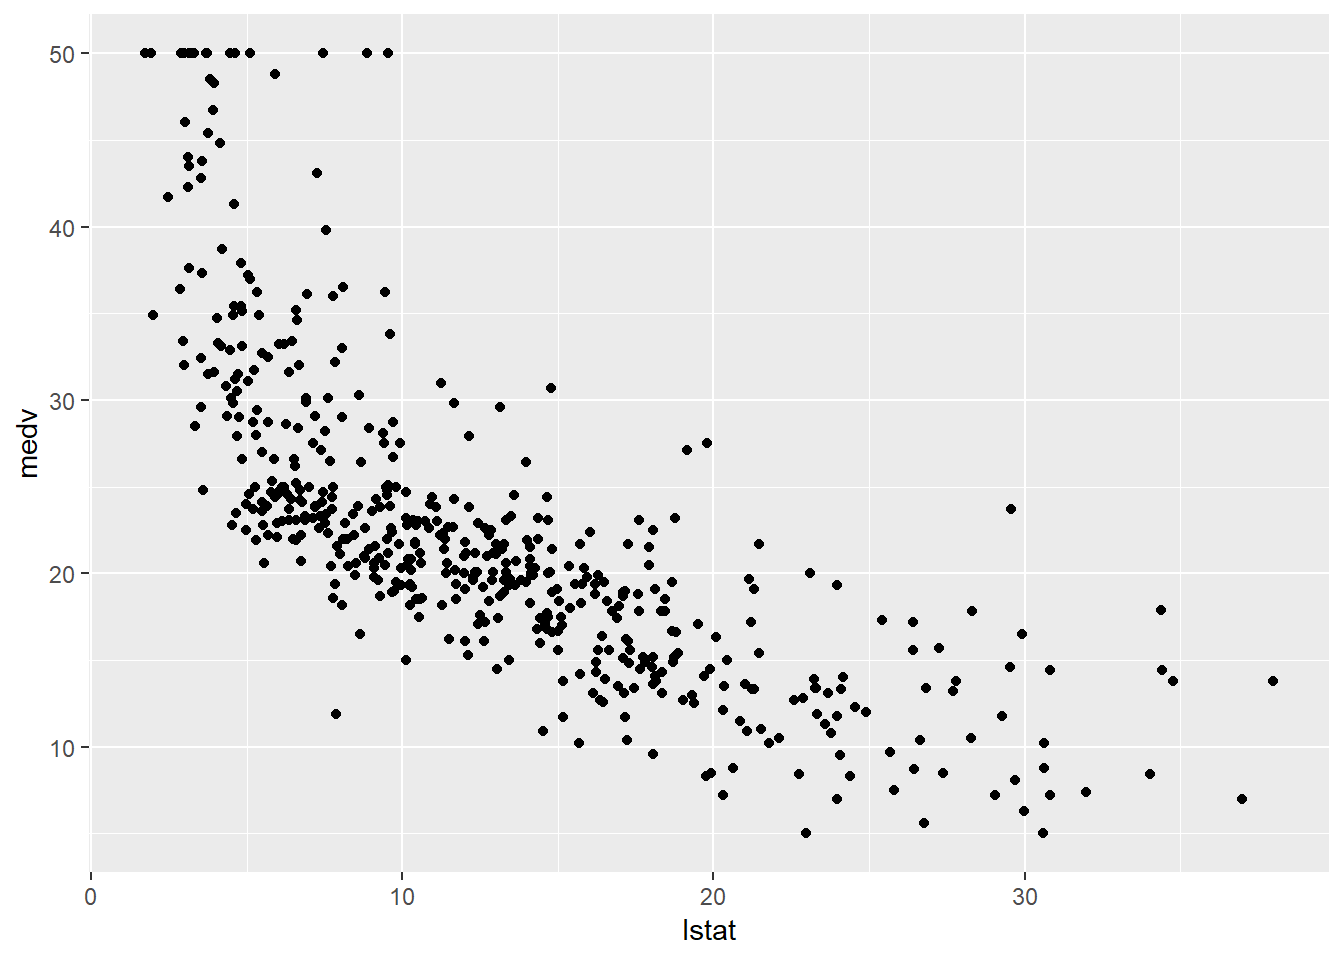
\includegraphics{Regression_files/figure-latex/unnamed-chunk-4-1.pdf}

\hypertarget{build-a-model-to-predict-medv}{%
\subsubsection{\texorpdfstring{Build a model to predict
\texttt{medv}}{Build a model to predict medv}}\label{build-a-model-to-predict-medv}}

Do single linear regression utilizing \texttt{lm}

\begin{Shaded}
\begin{Highlighting}[]
\NormalTok{model_}\DecValTok{1}\NormalTok{ =}\StringTok{ }\KeywordTok{lm}\NormalTok{(lstat }\OperatorTok{~}\StringTok{ }\NormalTok{medv, }\DataTypeTok{data =}\NormalTok{ data)}
\NormalTok{model_}\DecValTok{1}
\end{Highlighting}
\end{Shaded}

\begin{verbatim}
## 
## Call:
## lm(formula = lstat ~ medv, data = data)
## 
## Coefficients:
## (Intercept)         medv  
##     25.5589      -0.5728
\end{verbatim}

\hypertarget{show-a-better-description-of-the-model}{%
\subsubsection{Show a better description of the
model}\label{show-a-better-description-of-the-model}}

\begin{Shaded}
\begin{Highlighting}[]
\KeywordTok{summary}\NormalTok{(model_}\DecValTok{1}\NormalTok{)}
\end{Highlighting}
\end{Shaded}

\begin{verbatim}
## 
## Call:
## lm(formula = lstat ~ medv, data = data)
## 
## Residuals:
##      Min       1Q   Median       3Q      Max 
## -10.8631  -3.5959  -0.8133   2.4069  20.3152 
## 
## Coefficients:
##             Estimate Std. Error t value Pr(>|t|)    
## (Intercept) 25.55886    0.56823   44.98   <2e-16 ***
## medv        -0.57276    0.02335  -24.53   <2e-16 ***
## ---
## Signif. codes:  0 '***' 0.001 '**' 0.01 '*' 0.05 '.' 0.1 ' ' 1
## 
## Residual standard error: 4.826 on 504 degrees of freedom
## Multiple R-squared:  0.5441, Adjusted R-squared:  0.5432 
## F-statistic: 601.6 on 1 and 504 DF,  p-value: < 2.2e-16
\end{verbatim}

\hypertarget{interpret-what-your-results-above-mean}{%
\subsubsection{Interpret what your results above
mean:}\label{interpret-what-your-results-above-mean}}

\textless{} Homework \textgreater{}

This tells us that there is a strong statistical correlation between
lstat and medv.

\hypertarget{can-you-display-the-confidence-intervals}{%
\subsubsection{Can you display the confidence
intervals?}\label{can-you-display-the-confidence-intervals}}

\begin{Shaded}
\begin{Highlighting}[]
\KeywordTok{confint}\NormalTok{(model_}\DecValTok{1}\NormalTok{)}
\end{Highlighting}
\end{Shaded}

\begin{verbatim}
##                  2.5 %     97.5 %
## (Intercept) 24.4424687 26.6752498
## medv        -0.6186335 -0.5268781
\end{verbatim}

\hypertarget{interpret-what-your-results-above-mean-1}{%
\subsubsection{Interpret what your results above
mean:}\label{interpret-what-your-results-above-mean-1}}

\textless{} Homework \textgreater{}

I honestly don't know what is going on here

\hypertarget{predict-points-for-lstat-values-of-c5-10-15}{%
\subsubsection{Predict points for lstat values of c(5, 10,
15)}\label{predict-points-for-lstat-values-of-c5-10-15}}

\begin{Shaded}
\begin{Highlighting}[]
\NormalTok{predict_points =}\StringTok{ }\KeywordTok{tibble}\NormalTok{(}\DataTypeTok{lstat =} \KeywordTok{c}\NormalTok{(}\DecValTok{5}\NormalTok{, }\DecValTok{10}\NormalTok{, }\DecValTok{15}\NormalTok{))}
\KeywordTok{predict}\NormalTok{(model_}\DecValTok{1}\NormalTok{,  , }\DataTypeTok{interval=} \StringTok{'prediction'}\NormalTok{)}
\end{Highlighting}
\end{Shaded}

\begin{verbatim}
## Warning in predict.lm(model_1, , interval = "prediction"): predictions on current data refer to _future_ responses
\end{verbatim}

\begin{verbatim}
##            fit          lwr       upr
## 1   11.8127195   2.32115406 21.304285
## 2   13.1873335   3.69591023 22.678757
## 3    5.6842322  -3.82349484 15.191959
## 4    6.4288148  -3.07559721 15.933227
## 5    4.8250985  -4.68691690 14.337114
## 6    9.1207672  -0.37477585 18.616310
## 7   12.4427509   2.95140919 21.934093
## 8   10.0371765   0.54353714 19.530816
## 9   16.1083882   6.61302687 25.603749
## 10  14.7337742   5.24098425 24.226564
## 11  16.9675219   7.46990563 26.465138
## 12  14.7337742   5.24098425 24.226564
## 13  13.1300579   3.63865423 22.621462
## 14  13.8746405   4.38280934 23.366472
## 15  15.1347033   5.64129519 24.628111
## 16  14.1610184   4.66892307 23.653114
## 17  12.3281998   2.83683731 21.819562
## 18  15.5356324   6.04149754 25.029767
## 19  13.9891916   4.49726148 23.481122
## 20  15.1347033   5.64129519 24.628111
## 21  17.7693801   8.26920987 27.269550
## 22  14.3328451   4.84056470 23.825126
## 23  16.8529707   7.35568391 26.350258
## 24  17.2538998   7.75542121 26.752378
## 25  16.6238684   7.12721391 26.120523
## 26  17.5975533   8.09796689 27.097140
## 27  16.0511126   6.55588391 25.546341
## 28  17.0820731   7.58411850 26.580028
## 29  15.0201521   5.52693172 24.513373
## 30  13.5309870   4.03939970 23.022574
## 31  18.2848603   8.78281941 27.786901
## 32  17.2538998   7.75542121 26.752378
## 33  17.9984824   8.49750289 27.499462
## 34  18.0557580   8.55457061 27.556945
## 35  17.8266556   8.32628644 27.327025
## 36  14.7337742   5.24098425 24.226564
## 37  14.1037428   4.61170475 23.595781
## 38  13.5309870   4.03939970 23.022574
## 39  11.4117904   1.91994291 20.903638
## 40   7.9179799  -1.58092195 17.416882
## 41   5.5696811  -3.93858912 15.077951
## 42  10.3235544   0.83039363 19.816715
## 43  11.0681370   1.57596118 20.560313
## 44  11.4117904   1.91994291 20.903638
## 45  13.4164358   3.92491208 22.907960
## 46  14.5046719   5.01218638 23.997157
## 47  14.1037428   4.61170475 23.595781
## 48  16.0511126   6.55588391 25.546341
## 49  17.3111754   7.81251769 26.809833
## 50  14.4473963   4.95498137 23.939811
## 51  14.2755696   4.78335304 23.767786
## 52  13.8173649   4.32557994 23.309150
## 53  11.2399637   1.74796202 20.731965
## 54  12.1563730   2.66496285 21.647783
## 55  14.7337742   5.24098425 24.226564
## 56   5.2833032  -4.22636340 14.792970
## 57  11.4117904   1.91994291 20.903638
## 58   7.4597753  -2.04066286 16.960213
## 59  12.2136486   2.72225655 21.705041
## 60  14.3328451   4.84056470 23.825126
## 61  14.8483254   5.35536988 24.341281
## 62  16.3947661   6.89870848 25.890824
## 63  12.8436800   3.35234094 22.335019
## 64  11.2399637   1.74796202 20.731965
## 65   6.6579171  -2.84554993 16.161384
## 66  12.0990974   2.60766693 21.590528
## 67  14.4473963   4.95498137 23.939811
## 68  12.9582312   3.46687290 22.449589
## 69  15.5929079   6.09866044 25.087155
## 70  13.5882626   4.09664018 23.079885
## 71  11.6981684   2.20653339 21.189803
## 72  13.1300579   3.63865423 22.621462
## 73  12.5000265   3.00869181 21.991361
## 74  12.1563730   2.66496285 21.647783
## 75  11.7554439   2.26384483 21.247043
## 76  13.3018847   3.81041559 22.793354
## 77  14.1037428   4.61170475 23.595781
## 78  13.6455381   4.15387845 23.137198
## 79  13.4164358   3.92491208 22.907960
## 80  13.9319161   4.44003652 23.423796
## 81   9.5216962   0.02705586 19.016337
## 82  11.8699951   2.37846107 21.361529
## 83  11.3545149   1.86261817 20.846412
## 84  12.4427509   2.95140919 21.934093
## 85  11.8699951   2.37846107 21.361529
## 86  10.3235544   0.83039363 19.816715
## 87  12.6718533   3.18052635 22.163180
## 88  12.8436800   3.35234094 22.335019
## 89  12.0418219   2.55036879 21.533275
## 90   9.1207672  -0.37477585 18.616310
## 91  12.6145777   3.12325039 22.105905
## 92  12.9582312   3.46687290 22.449589
## 93  12.4427509   2.95140919 21.934093
## 94  11.2399637   1.74796202 20.731965
## 95  13.7600893   4.26834833 23.251830
## 96   9.2925939  -0.20254897 18.787737
## 97  13.3018847   3.81041559 22.793354
## 98   3.3932090  -6.12705484 12.913473
## 99   0.4721543  -9.06919019 10.013499
## 100  6.5433660  -2.96056915 16.047301
## 101  9.8080741   0.31401206 19.302136
## 102 10.3808300   0.88775828 19.873902
## 103 14.9056010   5.41255938 24.398643
## 104 14.5046719   5.01218638 23.997157
## 105 14.0464672   4.55448423 23.538450
## 106 14.3901207   4.89777414 23.882467
## 107 14.3901207   4.89777414 23.882467
## 108 13.8746405   4.38280934 23.366472
## 109 14.2182940   4.72613916 23.710449
## 110 14.4473963   4.95498137 23.939811
## 111 13.1300579   3.63865423 22.621462
## 112 12.5000265   3.00869181 21.991361
## 113 14.7910498   5.29817817 24.283921
## 114 14.8483254   5.35536988 24.341281
## 115 14.9628765   5.46974666 24.456006
## 116 15.0774277   5.58411456 24.570741
## 117 13.4164358   3.92491208 22.907960
## 118 14.5619475   5.06938917 24.054506
## 119 13.8746405   4.38280934 23.366472
## 120 14.5046719   5.01218638 23.997157
## 121 12.9582312   3.46687290 22.449589
## 122 13.9319161   4.44003652 23.423796
## 123 13.8173649   4.32557994 23.309150
## 124 15.6501835   6.15582113 25.144546
## 125 14.7910498   5.29817817 24.283921
## 126 13.3018847   3.81041559 22.793354
## 127 16.5665928   7.07009087 26.063095
## 128 16.2802149   6.78444248 25.775987
## 129 15.2492544   5.75564980 24.742859
## 130 17.3684510   7.86961195 26.867290
## 131 14.5619475   5.06938917 24.054506
## 132 14.3328451   4.84056470 23.825126
## 133 12.3854753   2.89412436 21.876826
## 134 15.0201521   5.52693172 24.513373
## 135 16.6238684   7.12721391 26.120523
## 136 15.1919789   5.69847360 24.685484
## 137 15.5929079   6.09866044 25.087155
## 138 15.7647347   6.27013586 25.259334
## 139 17.9412068   8.44043295 27.441981
## 140 15.3638056   5.86999554 24.857616
## 141 17.5402777   8.04088148 27.039674
## 142 17.3111754   7.81251769 26.809833
## 143 17.8839312   8.38336080 27.384502
## 144 16.6238684   7.12721391 26.120523
## 145 18.8003405   9.29624994 28.304431
## 146 17.6548289   8.15505010 27.154608
## 147 16.6238684   7.12721391 26.120523
## 148 17.1966242   7.69832252 26.694926
## 149 15.3638056   5.86999554 24.857616
## 150 16.7384196   7.24145334 26.235386
## 151 13.2446091   3.75316402 22.736054
## 152 14.3328451   4.84056470 23.825126
## 153 16.7956952   7.29856973 26.292821
## 154 14.4473963   4.95498137 23.939811
## 155 15.8220103   6.32728990 25.316731
## 156 16.6238684   7.12721391 26.120523
## 157 18.0557580   8.55457061 27.556945
## 158  1.9040438  -7.62625507 11.434343
## 159 11.6408928   2.14921973 21.132566
## 160 12.2136486   2.72225655 21.705041
## 161 10.0944521   0.60091287 19.587991
## 162 -3.0789318 -12.65354483  6.495681
## 163 -3.0789318 -12.65354483  6.495681
## 164 -3.0789318 -12.65354483  6.495681
## 165 12.5573021   3.06597221 22.048632
## 166 11.2399637   1.74796202 20.731965
## 167 -3.0789318 -12.65354483  6.495681
## 168 11.9272707   2.43576586 21.418776
## 169 11.9272707   2.43576586 21.418776
## 170 12.7864044   3.29507162 22.277737
## 171 15.5929079   6.09866044 25.087155
## 172 14.6192230   5.12658975 24.111856
## 173 12.3281998   2.83683731 21.819562
## 174 12.0418219   2.55036879 21.533275
## 175 12.6145777   3.12325039 22.105905
## 176  8.7198381  -0.77671608 18.216392
## 177 12.2709242   2.77954804 21.762300
## 178 11.4690660   1.97726544 20.960867
## 179  8.4334602  -1.06388267 17.930803
## 180  4.2523427  -5.26280703 13.767492
## 181  2.7631776  -6.76115084 12.287506
## 182  4.8250985  -4.68691690 14.337114
## 183  3.8514136  -5.66606110 13.368888
## 184  6.9442950  -2.55804054 16.446631
## 185 10.4381056   0.94512071 19.931090
## 186  8.6052869  -0.89157608 18.102150
## 187 -3.0789318 -12.65354483  6.495681
## 188  7.2306730  -2.27058639 16.731932
## 189  8.4907358  -1.00644493 17.987916
## 190  5.5696811  -3.93858912 15.077951
## 191  4.3668938  -5.14761139 13.881399
## 192  8.0898067  -1.40855561 17.588169
## 193  4.7105473  -4.80207731 14.223172
## 194  7.7461532  -1.75330821 17.245615
## 195  8.8916648  -0.60444270 18.387772
## 196 -3.0789318 -12.65354483  6.495681
## 197  6.4860904  -3.01808208 15.990263
## 198  8.2043579  -1.29365578 17.702371
## 199  5.7415078  -3.76595101 15.248967
## 200  5.5696811  -3.93858912 15.077951
## 201  6.7151927  -2.78804363 16.218429
## 202 11.7554439   2.26384483 21.247043
## 203  1.3312880  -8.20326509 10.865841
## 204 -2.2197981 -11.78559729  7.346001
## 205 -3.0789318 -12.65354483  6.495681
## 206 12.6145777   3.12325039 22.105905
## 207 11.5836172   2.09190385 21.075331
## 208 12.6718533   3.18052635 22.163180
## 209 11.5836172   2.09190385 21.075331
## 210 14.1037428   4.61170475 23.595781
## 211 13.1300579   3.63865423 22.621462
## 212 14.5046719   5.01218638 23.997157
## 213 12.7291288   3.23780010 22.220458
## 214  9.4644207  -0.03034202 18.959183
## 215 11.9845463   2.49306843 21.476024
## 216 11.2399637   1.74796202 20.731965
## 217 12.2136486   2.72225655 21.705041
## 218  9.1207672  -0.37477585 18.616310
## 219 13.2446091   3.75316402 22.736054
## 220 12.3854753   2.89412436 21.876826
## 221 10.2662788   0.77302676 19.759531
## 222 13.1300579   3.63865423 22.621462
## 223  9.8080741   0.31401206 19.302136
## 224  8.3189090  -1.17876480 17.816583
## 225 -0.1006016  -9.64674651  9.445543
## 226 -3.0789318 -12.65354483  6.495681
## 227  4.0232404  -5.49322473 13.539705
## 228  7.4597753  -2.04066286 16.960213
## 229 -1.1888376 -10.74470370  8.367028
## 230  7.5170509  -1.98318751 17.017289
## 231 11.6408928   2.14921973 21.132566
## 232  7.4024997  -2.09814043 16.903140
## 233  1.6749415  -7.85703281 11.206916
## 234 -2.1052469 -11.66990775  7.459414
## 235  8.9489404  -0.54702267 18.444904
## 236 11.8127195   2.32115406 21.304285
## 237 11.1826881   1.69063062 20.674746
## 238  7.5170509  -1.98318751 17.017289
## 239 11.9845463   2.49306843 21.476024
## 240 12.2136486   2.72225655 21.705041
## 241 12.9582312   3.46687290 22.449589
## 242 14.0464672   4.55448423 23.538450
## 243 12.8436800   3.35234094 22.335019
## 244 11.9845463   2.49306843 21.476024
## 245 15.4783568   5.98433243 24.972381
## 246 14.9628765   5.46974666 24.456006
## 247 11.6408928   2.14921973 21.132566
## 248 13.8173649   4.32557994 23.309150
## 249 11.5263416   2.03458576 21.018097
## 250 10.5526567   1.05983893 20.045475
## 251 11.5836172   2.09190385 21.075331
## 252 11.3545149   1.86261817 20.846412
## 253  8.6052869  -0.89157608 18.102150
## 254  1.0449101  -8.49185215 10.581672
## 255 13.0155067   3.52413556 22.506878
## 256 13.5882626   4.09664018 23.079885
## 257  0.3576031  -9.18468400  9.899890
## 258 -3.0789318 -12.65354483  6.495681
## 259  4.9396497  -4.57176530 14.451065
## 260  8.3189090  -1.17876480 17.816583
## 261  6.1997125  -3.30567983 15.705105
## 262  0.8730833  -8.66503062 10.411197
## 263 -2.3916248 -11.95914785  7.175898
## 264  7.8034288  -1.69584391 17.302701
## 265  4.6532718  -4.85966082 14.166204
## 266 12.5000265   3.00869181 21.991361
## 267  7.9752555  -1.52346429 17.473975
## 268 -3.0789318 -12.65354483  6.495681
## 269  0.6439810  -8.89596584 10.183928
## 270 13.7028137   4.21111450 23.194513
## 271 13.4737114   3.98215700 22.965266
## 272 11.1254125   1.63329701 20.617528
## 273 11.5836172   2.09190385 21.075331
## 274  5.3978543  -4.11124707 14.906956
## 275  7.0015706  -2.50054529 16.503687
## 276  7.2306730  -2.27058639 16.731932
## 277  6.5433660  -2.96056915 16.047301
## 278  6.6006416  -2.90305844 16.104342
## 279  8.8916648  -0.60444270 18.387772
## 280  5.4551299  -4.05369222 14.963952
## 281 -0.4442550  -9.99338494  9.104875
## 282  5.2833032  -4.22636340 14.792970
## 283 -0.7879085 -10.34010177  8.764285
## 284 -3.0789318 -12.65354483  6.495681
## 285  7.1161218  -2.38556142 16.617805
## 286 12.9582312   3.46687290 22.449589
## 287 14.0464672   4.55448423 23.538450
## 288 12.2709242   2.77954804 21.762300
## 289 12.7864044   3.29507162 22.277737
## 290 11.3545149   1.86261817 20.846412
## 291  9.2353183  -0.25995572 18.730592
## 292  4.1950671  -5.32040816 13.710542
## 293  9.5789718   0.08445153 19.073492
## 294 11.8699951   2.37846107 21.361529
## 295 13.1300579   3.63865423 22.621462
## 296  9.1780427  -0.31736468 18.673450
## 297 10.0371765   0.54353714 19.530816
## 298 13.9319161   4.44003652 23.423796
## 299 12.6718533   3.18052635 22.163180
## 300  8.9489404  -0.54702267 18.444904
## 301 11.3545149   1.86261817 20.846412
## 302 12.9582312   3.46687290 22.449589
## 303 10.4381056   0.94512071 19.931090
## 304  6.6006416  -2.90305844 16.104342
## 305  4.8823741  -4.62934000 14.394088
## 306  9.2925939  -0.20254897 18.787737
## 307  6.4288148  -3.07559721 15.933227
## 308  9.4071451  -0.08774212 18.902032
## 309 12.5000265   3.00869181 21.991361
## 310 13.9319161   4.44003652 23.423796
## 311 16.3374905   6.84157659 25.833404
## 312 12.9009556   3.40960803 22.392303
## 313 14.4473963   4.95498137 23.939811
## 314 13.1873335   3.69591023 22.678757
## 315 11.9272707   2.43576586 21.418776
## 316 16.2802149   6.78444248 25.775987
## 317 15.3638056   5.86999554 24.857616
## 318 14.2182940   4.72613916 23.710449
## 319 12.3281998   2.83683731 21.819562
## 320 13.5309870   4.03939970 23.022574
## 321 11.9272707   2.43576586 21.418776
## 322 12.3281998   2.83683731 21.819562
## 323 13.8746405   4.38280934 23.366472
## 324 14.9628765   5.46974666 24.456006
## 325 11.2399637   1.74796202 20.731965
## 326 11.4690660   1.97726544 20.960867
## 327 12.3854753   2.89412436 21.876826
## 328 12.8436800   3.35234094 22.335019
## 329 14.5046719   5.01218638 23.997157
## 330 12.6145777   3.12325039 22.105905
## 331 14.2182940   4.72613916 23.710449
## 332 15.7647347   6.27013586 25.259334
## 333 14.4473963   4.95498137 23.939811
## 334 12.8436800   3.35234094 22.335019
## 335 13.7028137   4.21111450 23.194513
## 336 13.4737114   3.98215700 22.965266
## 337 14.3901207   4.89777414 23.882467
## 338 14.9628765   5.46974666 24.456006
## 339 13.7600893   4.26834833 23.251830
## 340 14.6764986   5.18378811 24.169209
## 341 14.8483254   5.35536988 24.341281
## 342  6.8297439  -2.67303767 16.332525
## 343 16.1083882   6.61302687 25.603749
## 344 11.8699951   2.37846107 21.361529
## 345  7.6888776  -1.81077471 17.188530
## 346 15.5356324   6.04149754 25.029767
## 347 15.7074591   6.21297960 25.201939
## 348 12.3281998   2.83683731 21.819562
## 349 11.5263416   2.03458576 21.018097
## 350 10.3235544   0.83039363 19.816715
## 351 12.4427509   2.95140919 21.934093
## 352 11.7554439   2.26384483 21.247043
## 353 14.9056010   5.41255938 24.398643
## 354  8.3189090  -1.17876480 17.816583
## 355 15.1347033   5.64129519 24.628111
## 356 13.7600893   4.26834833 23.251830
## 357 15.3638056   5.86999554 24.857616
## 358 13.1300579   3.63865423 22.621462
## 359 12.5573021   3.06597221 22.048632
## 360 12.6145777   3.12325039 22.105905
## 361 11.2399637   1.74796202 20.731965
## 362 14.1610184   4.66892307 23.653114
## 363 13.6455381   4.15387845 23.137198
## 364 15.9365614   6.44159133 25.431532
## 365 13.0155067   3.52413556 22.506878
## 366  9.8080741   0.31401206 19.302136
## 367 13.0155067   3.52413556 22.506878
## 368 12.3281998   2.83683731 21.819562
## 369 -3.0789318 -12.65354483  6.495681
## 370 -3.0789318 -12.65354483  6.495681
## 371 -3.0789318 -12.65354483  6.495681
## 372 -3.0789318 -12.65354483  6.495681
## 373 -3.0789318 -12.65354483  6.495681
## 374 17.6548289   8.15505010 27.154608
## 375 17.6548289   8.15505010 27.154608
## 376 16.9675219   7.46990563 26.465138
## 377 17.5975533   8.09796689 27.097140
## 378 17.9412068   8.44043295 27.441981
## 379 18.0557580   8.55457061 27.556945
## 380 19.7167499  10.20857367 29.224926
## 381 19.6021987  10.09456410 29.109833
## 382 19.3158208   9.80950156 28.822140
## 383 19.0867184   9.58141181 28.592025
## 384 18.5139626   9.01103285 28.016892
## 385 20.5186080  11.00639370 30.030822
## 386 21.4350173  11.91765934 30.952375
## 387 19.5449231  10.03755601 29.052290
## 388 21.3204662  11.80378194 30.837150
## 389 19.7167499  10.20857367 29.224926
## 390 18.9721673   9.46735368 28.476981
## 391 16.9102463   7.41279588 26.407697
## 392 12.2709242   2.77954804 21.762300
## 393 20.0031278  10.49355900 29.512697
## 394 17.6548289   8.15505010 27.154608
## 395 18.2848603   8.78281941 27.786901
## 396 18.0557580   8.55457061 27.556945
## 397 18.3994115   8.89693055 27.901892
## 398 20.6904347  11.17729894 30.203571
## 399 22.6950801  13.16973046 32.220430
## 400 21.9504976  12.42999877 31.470996
## 401 22.3514266  12.82836194 31.874491
## 402 21.4350173  11.91765934 30.952375
## 403 18.6285138   9.12512631 28.131901
## 404 20.8049859  11.29122475 30.318747
## 405 20.6904347  11.17729894 30.203571
## 406 22.6950801  13.16973046 32.220430
## 407 18.7430650   9.23921094 28.246919
## 408  9.5789718   0.08445153 19.073492
## 409 15.7074591   6.21297960 25.201939
## 410  9.8080741   0.31401206 19.302136
## 411 16.9675219   7.46990563 26.465138
## 412 15.7074591   6.21297960 25.201939
## 413 15.3065300   5.81282378 24.800236
## 414 16.2229393   6.72730616 25.718573
## 415 21.5495685  12.03152794 31.067609
## 416 21.4350173  11.91765934 30.952375
## 417 21.2631906  11.74683995 30.779541
## 418 19.6021987  10.09456410 29.109833
## 419 20.5186080  11.00639370 30.030822
## 420 20.7477103  11.23426294 30.261158
## 421 15.9938370   6.49873873 25.488935
## 422 17.4257266   7.92670401 26.924749
## 423 13.6455381   4.15387845 23.137198
## 424 17.8839312   8.38336080 27.384502
## 425 18.8576161   9.35328673 28.361946
## 426 20.8049859  11.29122475 30.318747
## 427 19.7167499  10.20857367 29.224926
## 428 19.3158208   9.80950156 28.822140
## 429 19.2585452   9.75248244 28.764608
## 430 20.1176789  10.60753769 29.627820
## 431 17.2538998   7.75542121 26.752378
## 432 17.4830022   7.98379385 26.982210
## 433 16.3374905   6.84157659 25.833404
## 434 17.3684510   7.86961195 26.867290
## 435 18.8576161   9.35328673 28.361946
## 436 17.8839312   8.38336080 27.384502
## 437 20.0604033  10.55054945 29.570257
## 438 20.5758836  11.06336431 30.088403
## 439 20.7477103  11.23426294 30.261158
## 440 18.2275847   8.72576053 27.729409
## 441 19.5449231  10.03755601 29.052290
## 442 15.7647347   6.27013586 25.259334
## 443 15.0201521   5.52693172 24.513373
## 444 16.7384196   7.24145334 26.235386
## 445 19.3730964   9.86651848 28.879674
## 446 18.8003405   9.29624994 28.304431
## 447 17.0247975   7.52701318 26.522582
## 448 18.3421359   8.83987609 27.844396
## 449 17.4830022   7.98379385 26.982210
## 450 18.1130336   8.61163613 27.614431
## 451 17.8839312   8.38336080 27.384502
## 452 16.8529707   7.35568391 26.350258
## 453 16.3374905   6.84157659 25.833404
## 454 15.3638056   5.86999554 24.857616
## 455 17.0247975   7.52701318 26.522582
## 456 17.4830022   7.98379385 26.982210
## 457 18.2848603   8.78281941 27.786901
## 458 17.8266556   8.32628644 27.327025
## 459 17.0247975   7.52701318 26.522582
## 460 14.1037428   4.61170475 23.595781
## 461 16.1656638   6.67016762 25.661160
## 462 15.4210812   5.92716509 24.914997
## 463 14.3901207   4.89777414 23.882467
## 464 13.9891916   4.49726148 23.481122
## 465 13.3018847   3.81041559 22.793354
## 466 14.1610184   4.66892307 23.653114
## 467 14.6764986   5.18378811 24.169209
## 468 14.6192230   5.12658975 24.111856
## 469 14.6192230   5.12658975 24.111856
## 470 14.0464672   4.55448423 23.538450
## 471 14.1610184   4.66892307 23.653114
## 472 14.3328451   4.84056470 23.825126
## 473 12.2709242   2.77954804 21.762300
## 474  8.4907358  -1.00644493 17.987916
## 475 17.6548289   8.15505010 27.154608
## 476 17.9412068   8.44043295 27.441981
## 477 15.9938370   6.49873873 25.488935
## 478 18.6857894   9.18216973 28.189409
## 479 17.1966242   7.69832252 26.694926
## 480 13.3018847   3.81041559 22.793354
## 481 12.3854753   2.89412436 21.876826
## 482 11.9845463   2.49306843 21.476024
## 483 11.2399637   1.74796202 20.731965
## 484 13.0727823   3.58139600 22.564169
## 485 13.7600893   4.26834833 23.251830
## 486 13.4164358   3.92491208 22.907960
## 487 14.6192230   5.12658975 24.111856
## 488 13.7600893   4.26834833 23.251830
## 489 16.8529707   7.35568391 26.350258
## 490 21.5495685  12.03152794 31.067609
## 491 20.9195371  11.40514176 30.433932
## 492 17.7693801   8.26920987 27.269550
## 493 14.0464672   4.55448423 23.538450
## 494 13.0727823   3.58139600 22.564169
## 495 11.5263416   2.03458576 21.018097
## 496 12.3281998   2.83683731 21.819562
## 497 14.2755696   4.78335304 23.767786
## 498 15.0774277   5.58411456 24.570741
## 499 13.4164358   3.92491208 22.907960
## 500 15.5356324   6.04149754 25.029767
## 501 15.9365614   6.44159133 25.431532
## 502 12.7291288   3.23780010 22.220458
## 503 13.7600893   4.26834833 23.251830
## 504 11.8699951   2.37846107 21.361529
## 505 12.9582312   3.46687290 22.449589
## 506 18.7430650   9.23921094 28.246919
\end{verbatim}

\hypertarget{plot-your-first-model}{%
\subsubsection{Plot your first model}\label{plot-your-first-model}}

\begin{Shaded}
\begin{Highlighting}[]
\KeywordTok{ggPredict}\NormalTok{(model_}\DecValTok{1}\NormalTok{)}\OperatorTok{+}
\StringTok{  }\KeywordTok{geom_smooth}\NormalTok{()}
\end{Highlighting}
\end{Shaded}

\begin{verbatim}
## `geom_smooth()` using method = 'loess' and formula 'y ~ x'
\end{verbatim}

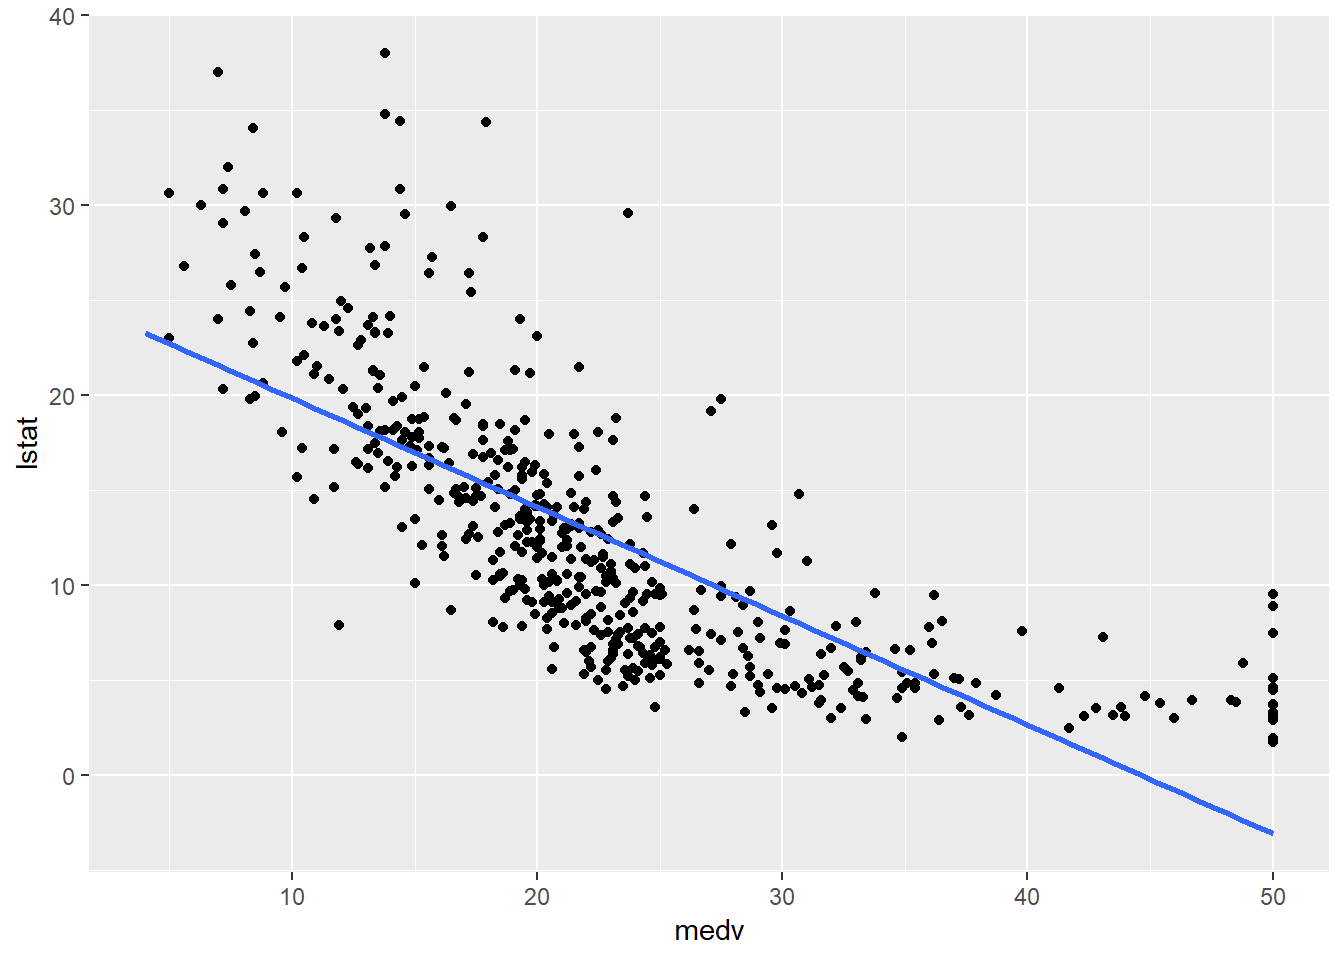
\includegraphics{Regression_files/figure-latex/unnamed-chunk-9-1.pdf}

\hypertarget{create-a-model-using-both-lstat-and-age}{%
\subsubsection{\texorpdfstring{Create a model using both \texttt{lstat}
and
\texttt{age}}{Create a model using both lstat and age}}\label{create-a-model-using-both-lstat-and-age}}

\begin{Shaded}
\begin{Highlighting}[]
\NormalTok{model_}\DecValTok{2}\NormalTok{ =}\StringTok{ }\KeywordTok{lm}\NormalTok{(lstat }\OperatorTok{~}\StringTok{ }\NormalTok{age, }\DataTypeTok{data =}\NormalTok{ data)}
\KeywordTok{summary}\NormalTok{(model_}\DecValTok{2}\NormalTok{)}
\end{Highlighting}
\end{Shaded}

\begin{verbatim}
## 
## Call:
## lm(formula = lstat ~ age, data = data)
## 
## Residuals:
##      Min       1Q   Median       3Q      Max 
## -15.2600  -3.3552  -0.1492   2.6266  25.8781 
## 
## Coefficients:
##             Estimate Std. Error t value Pr(>|t|)    
## (Intercept)  2.17435    0.66856   3.252  0.00122 ** 
## age          0.15281    0.00902  16.940  < 2e-16 ***
## ---
## Signif. codes:  0 '***' 0.001 '**' 0.01 '*' 0.05 '.' 0.1 ' ' 1
## 
## Residual standard error: 5.706 on 504 degrees of freedom
## Multiple R-squared:  0.3628, Adjusted R-squared:  0.3615 
## F-statistic:   287 on 1 and 504 DF,  p-value: < 2.2e-16
\end{verbatim}

\hypertarget{interpret-what-your-results-above-mean-2}{%
\subsubsection{Interpret what your results above
mean:}\label{interpret-what-your-results-above-mean-2}}

\textless{} Homework \textgreater{}

That there is also a strong statistical correlation between lstat and
age. I feel okay about this model. The Multiple R-squared and adjusted
R-squared aren't great. the p-value

\hypertarget{create-a-model-using-all-variables-as-predictors}{%
\subsubsection{Create a model using all variables as
predictors}\label{create-a-model-using-all-variables-as-predictors}}

\begin{Shaded}
\begin{Highlighting}[]
\NormalTok{model_}\DecValTok{3}\NormalTok{ =}\StringTok{ }\KeywordTok{lm}\NormalTok{(lstat }\OperatorTok{~}\NormalTok{., }\DataTypeTok{data =}\NormalTok{ data)}
\KeywordTok{summary}\NormalTok{(model_}\DecValTok{3}\NormalTok{)}
\end{Highlighting}
\end{Shaded}

\begin{verbatim}
## 
## Call:
## lm(formula = lstat ~ ., data = data)
## 
## Residuals:
##      Min       1Q   Median       3Q      Max 
## -13.4344  -2.2498  -0.5345   1.9152  20.0091 
## 
## Coefficients:
##              Estimate Std. Error t value Pr(>|t|)    
## (Intercept) 37.155876   3.981340   9.333  < 2e-16 ***
## crim         0.044485   0.026690   1.667  0.09621 .  
## zn           0.027621   0.011117   2.484  0.01330 *  
## indus        0.082877   0.049406   1.677  0.09409 .  
## chas         0.085799   0.700912   0.122  0.90262    
## nox         -1.797038   3.143107  -0.572  0.56776    
## rm          -2.322790   0.348622  -6.663 7.22e-11 ***
## age          0.073206   0.010117   7.236 1.79e-12 ***
## dis         -0.378356   0.168523  -2.245  0.02520 *  
## rad          0.142536   0.054213   2.629  0.00883 ** 
## tax         -0.005134   0.003054  -1.681  0.09336 .  
## ptratio     -0.228266   0.110452  -2.067  0.03929 *  
## black       -0.003573   0.002184  -1.636  0.10253    
## medv        -0.340572   0.032915 -10.347  < 2e-16 ***
## ---
## Signif. codes:  0 '***' 0.001 '**' 0.01 '*' 0.05 '.' 0.1 ' ' 1
## 
## Residual standard error: 3.823 on 492 degrees of freedom
## Multiple R-squared:  0.7208, Adjusted R-squared:  0.7134 
## F-statistic:  97.7 on 13 and 492 DF,  p-value: < 2.2e-16
\end{verbatim}

\hypertarget{interpret-what-your-results-above-mean-3}{%
\subsubsection{Interpret what your results above
mean:}\label{interpret-what-your-results-above-mean-3}}

\textless{} Homework \textgreater{}

The strongest correlations are medv, age, rm. rad, dis, zn and ptratio
also are strongly correlated. Very good Multiple R-squared and Adjusted
R-squared values. There are better models in this assignment if I am
only looking at the F-statistic. But I would feel very good about this
model overall.

\hypertarget{how-do-these-numbers-compare-with-those-from-model_2}{%
\subsubsection{\texorpdfstring{How do these numbers compare with those
from \texttt{model\_2}
?}{How do these numbers compare with those from model\_2 ?}}\label{how-do-these-numbers-compare-with-those-from-model_2}}

\textless{} Homework \textgreater{}

Model 2

age 0.15281 0.00902 16.940 \textless{} 2e-16 ***

Model 3

age 0.073206 0.010117 7.236 1.79e-12 ***

\hypertarget{create-a-model-with-an-interaction-term}{%
\subsubsection{Create a model with an interaction
term}\label{create-a-model-with-an-interaction-term}}

Use \texttt{lstat} and \texttt{age} to predict \texttt{medv}

\begin{Shaded}
\begin{Highlighting}[]
\NormalTok{model_}\DecValTok{4}\NormalTok{ =}\StringTok{ }\KeywordTok{lm}\NormalTok{(medv }\OperatorTok{~}\StringTok{ }\NormalTok{lstat }\OperatorTok{+}\StringTok{ }\NormalTok{age, lstat}\OperatorTok{*}\NormalTok{age, }\DataTypeTok{data =}\NormalTok{ data)}
\KeywordTok{summary}\NormalTok{(model_}\DecValTok{4}\NormalTok{)}
\end{Highlighting}
\end{Shaded}

\begin{verbatim}
## 
## Call:
## lm(formula = medv ~ lstat + age, data = data, subset = lstat * 
##     age)
## 
## Residuals:
##     Min      1Q  Median      3Q     Max 
## -15.926  -3.618  -1.002   1.814  23.000 
## 
## Coefficients:
##             Estimate Std. Error t value Pr(>|t|)    
## (Intercept) 34.02079    1.07525   31.64   <2e-16 ***
## lstat       -1.07164    0.08332  -12.86   <2e-16 ***
## age          0.02785    0.01947    1.43    0.154    
## ---
## Signif. codes:  0 '***' 0.001 '**' 0.01 '*' 0.05 '.' 0.1 ' ' 1
## 
## Residual standard error: 5.755 on 182 degrees of freedom
##   (321 observations deleted due to missingness)
## Multiple R-squared:  0.5888, Adjusted R-squared:  0.5843 
## F-statistic: 130.3 on 2 and 182 DF,  p-value: < 2.2e-16
\end{verbatim}

\hypertarget{interpret-what-your-results-above-mean-4}{%
\subsubsection{Interpret what your results above
mean:}\label{interpret-what-your-results-above-mean-4}}

\textless{} Homework \textgreater{}

This is a good model. I can tell by the PR codes and the

\hypertarget{create-a-model-using-lstat-and-lstat-2}{%
\subsubsection{\texorpdfstring{Create a model using \texttt{lstat} and
\texttt{lstat\ \^{}\ 2}}{Create a model using lstat and lstat \^{} 2}}\label{create-a-model-using-lstat-and-lstat-2}}

\begin{Shaded}
\begin{Highlighting}[]
\NormalTok{model_}\DecValTok{5}\NormalTok{ =}\StringTok{ }\KeywordTok{lm}\NormalTok{(medv }\OperatorTok{~}\StringTok{ }\NormalTok{lstat }\OperatorTok{+}\StringTok{ }\KeywordTok{I}\NormalTok{(lstat}\OperatorTok{^}\DecValTok{2}\NormalTok{), }\DataTypeTok{data =}\NormalTok{ data)}
\KeywordTok{summary}\NormalTok{(model_}\DecValTok{5}\NormalTok{)}
\end{Highlighting}
\end{Shaded}

\begin{verbatim}
## 
## Call:
## lm(formula = medv ~ lstat + I(lstat^2), data = data)
## 
## Residuals:
##      Min       1Q   Median       3Q      Max 
## -15.2834  -3.8313  -0.5295   2.3095  25.4148 
## 
## Coefficients:
##              Estimate Std. Error t value Pr(>|t|)    
## (Intercept) 42.862007   0.872084   49.15   <2e-16 ***
## lstat       -2.332821   0.123803  -18.84   <2e-16 ***
## I(lstat^2)   0.043547   0.003745   11.63   <2e-16 ***
## ---
## Signif. codes:  0 '***' 0.001 '**' 0.01 '*' 0.05 '.' 0.1 ' ' 1
## 
## Residual standard error: 5.524 on 503 degrees of freedom
## Multiple R-squared:  0.6407, Adjusted R-squared:  0.6393 
## F-statistic: 448.5 on 2 and 503 DF,  p-value: < 2.2e-16
\end{verbatim}

\hypertarget{interpret-what-your-results-above-mean-5}{%
\subsubsection{Interpret what your results above
mean:}\label{interpret-what-your-results-above-mean-5}}

I can tell this is an even better model than model 4 because our
Multiple R-squared, Adjusted R-squared, F-statistic all improved while
the p-value stayed at \textless{}2.2e-16 which is really good.

\hypertarget{is-your-model-still-linear}{%
\subsubsection{Is your model still
linear?}\label{is-your-model-still-linear}}

\textless{} Homework \textgreater{}

\hypertarget{plot-your-models-fitted-values}{%
\subsubsection{Plot your model's fitted
values}\label{plot-your-models-fitted-values}}

The tibble \texttt{data\_model} has been created for you with the
predictions in a column called \texttt{medv\_predictions}

\begin{Shaded}
\begin{Highlighting}[]
\NormalTok{data_model =}\StringTok{ }\NormalTok{data }\OperatorTok
\StringTok{  }\KeywordTok{mutate}\NormalTok{(}\DataTypeTok{medv_predictions =} \KeywordTok{fitted}\NormalTok{(model_}\DecValTok{5}\NormalTok{))}

\NormalTok{data_model }\OperatorTok
\StringTok{  }\KeywordTok{ggplot}\NormalTok{(}\KeywordTok{aes}\NormalTok{(}\DataTypeTok{x=}\NormalTok{lstat)) }\OperatorTok{+}
\StringTok{  }\KeywordTok{geom_point}\NormalTok{(}\KeywordTok{aes}\NormalTok{(}\DataTypeTok{y=}\NormalTok{medv)) }\OperatorTok{+}\StringTok{ }
\StringTok{  }\KeywordTok{geom_point}\NormalTok{(}\KeywordTok{aes}\NormalTok{(}\DataTypeTok{y=}\NormalTok{medv_predictions), }\DataTypeTok{color=}\StringTok{'red'}\NormalTok{)}
\end{Highlighting}
\end{Shaded}

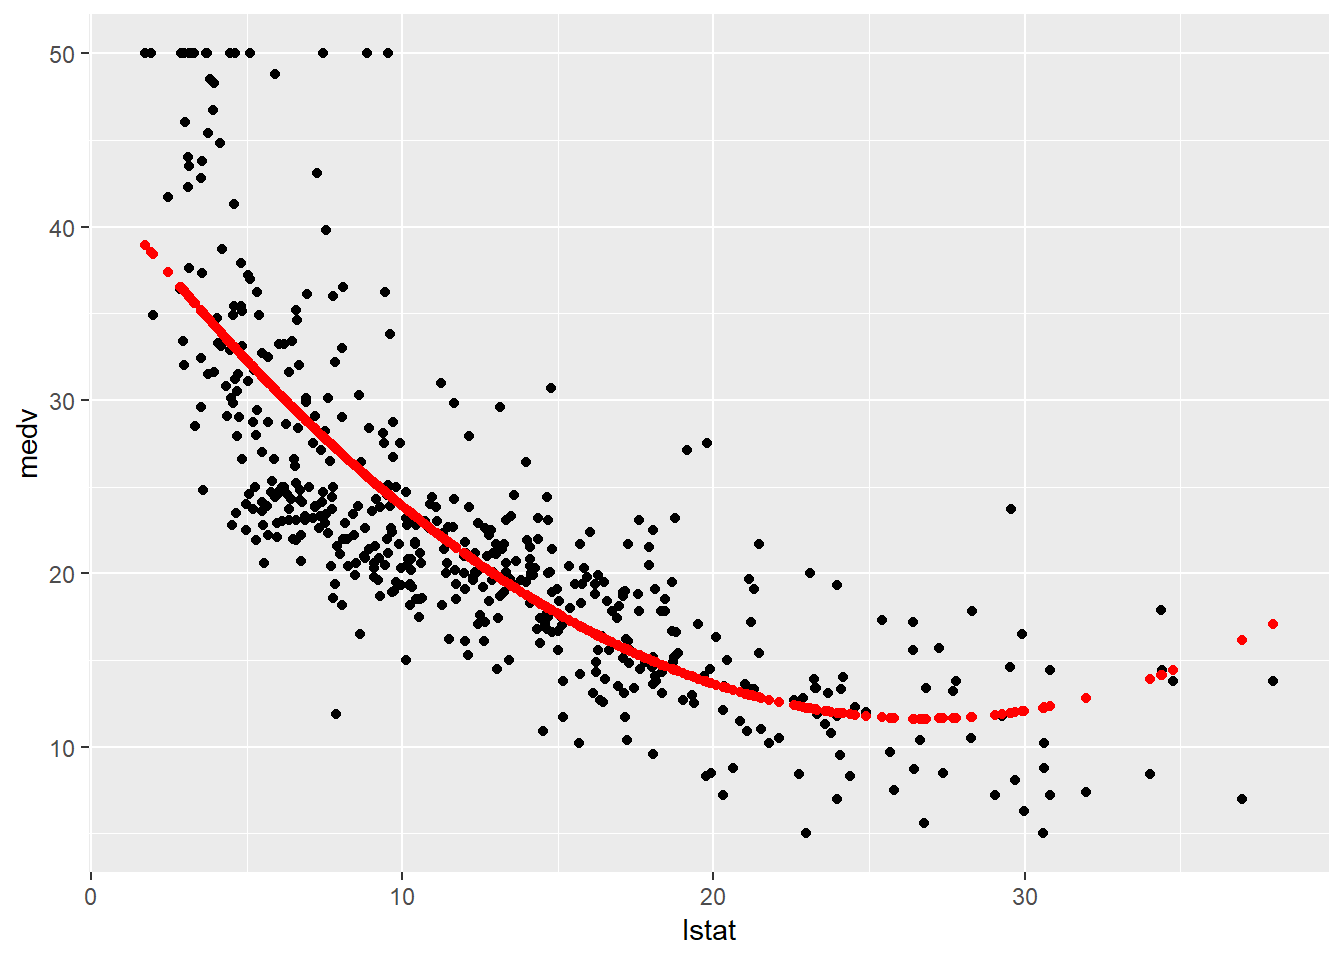
\includegraphics{Regression_files/figure-latex/unnamed-chunk-14-1.pdf}

\hypertarget{interpret-what-your-results-above-mean-6}{%
\subsubsection{Interpret what your results above
mean:}\label{interpret-what-your-results-above-mean-6}}

\textless{} Homework \textgreater{}

The black dots are the actual intersects of medv and lstat where the red
dots (which form a curved line) show where the intersects would be if
they perfectly matched the model.


\end{document}
